%--------------------------------------------------------------------------------------------------
\chapter{Umsetzung des Konzepts mit Hilfe der Unity Enginge}\label{cha:Umsetzung}
In diesem Kapitel wird die Umsetzung des Menschmodells und der Interaktion in der Entwicklungsumgebung der Unity Engine vorgestellt. Daher gibt es zunächst einen Einblick in die genutzte Hardware und Software, bevor das Menschmodell und die Interaktionsschnittstelle genauer erläutert werden.
%--------------------------------------------------------------------------------------------------
\section{Eingesetzte Hardware}\label{sec:Hardware}
Für die Umsetzung dieses Projektes wurde die Virtual Reality Brille \textbf{VIVE Pro} (Vgl. Abbildung \ref{fig:ViveproKit}) vom Hersteller HTC verwendet, da sie eine der Leistungsstärksten Brillen auf dem Markt ist. Zu den Stärken dieser Brille gehören das kontrastreiche OLED-Display, die sehr hohe Auflösung von 1440 x 1600 Pixeln pro Auge, eine Bildwiederholrate von 90Hz, ein Sichtfeld von 110 Grad und vor allem die Möglichkeit die Brille mit Hilfe des \textbf{Vive Wireless Sets} (Vgl. Abbildung \ref{fig:WirelessKit}) kabellos zu verwenden. Es ist anzumerken, dass für das kabellose Verwenden dieser VR Brille eine \textbf{Erweiterungskarte} in den PC eingebaut werden muss um einen speziellen \textbf{Empfänger} für die Signale der Brille anzuschließen. Des Weiteren muss ein \textbf{Sender} an der VR-Brille angebracht werden, welcher mit dem am PC angeschlossenen Empfänger kommuniziert und durch einen \textbf{mobilen Akku} mit Strom versorgt wird. Der mitgelieferte mobile Akku ermöglicht einen kabellosen Einsatz der VR Brille für bis zu sechs Stunden (Vgl. Abbildung \ref{fig:WirelessKit}) [28, ViveWeb].
\newline\newline
Um die Brille zu verwenden bedarf es mindesten zwei der sogenannten \textbf{SteamVR 2.0 Basisstationen} (Vgl. Abbildung \ref{fig:ViveproKit}), welche dem Bediener in Kombination mit des Vive Wireless Adapters eine enorme Bewegungsfreiheit ermöglichen. Beim Einsatz von zwei solcher Basisstationen ist eine Raumgröße von bis zu 5m x 5m, also 25m² möglich. Es ist sogar möglich bis zu vier solcher Basisstationen zu Verwenden und somit eine Raumgröße von bis zu 10m x 10m, also 100m² zu unterstützen [28, ViveWeb].
\newline\newline
Ein weiteres notwendiges Zubehör der Brille sind die beiden \textbf{Controller} (Vgl. Abbildung \ref{fig:ViveproKit}), die es dem Bediener ermöglichen mit der virtuellen Umgebung zu interagieren. Beide Controller werden wie die VR Brille durch die Basisstationen im Raum geortet und liefern Informationen über ihre eigene Position und Ausrichtung im Raum. Zusätzlich verfügen beide Controller über jeweils fünf Tasten, welche man mit eigenen Funktionalitäten versehen kann. Es ist anzumerken, dass die Tasten alle unterschiedlich sind und daher für unterschiedliche Zwecke verwendet werden können [29, ViveController].
\newline
Auf der Vorderseite der Controller befinden sich insgesamt drei Tasten [29, ViveController]:
\begin{itemize}
	\item Die erste dieser Tasten (ganz unten) ist die Taste um das Hauptmenü aufzurufen. Diese 
	Taste wird in der Regel nicht überschrieben und behält diese Funktionalität bei.
	\item Die zweite Taste (mittig) ist gleichzeitig ein Berührungsempfindliches Trackpad. Dem 
	Entwickler steht es frei, ob er diese Taste als einfache Taste oder als Trackpad verwenden 
	möchte. Es ist sogar Möglich beide Funktionen gleichzeitig in einer Anwendung zu 
	unterstützen. Dadurch eröffnen sich viele Anwendungsmöglichkeiten für diese Taste.
	\item Die dritte Taste (oben) ist wiederrum eine ganz einfache Taste und wird in den meisten 
	Anwendungen als eine einfache Menü-Taste verwendet.
\end{itemize}
Auf der Rückseite und der Außenseite des Controllers befinden sich zwei weitere Tasten [29, ViveController]:
\begin{itemize}
	\item Die Tasten links und rechts an der Außenseite des Controllers bilden eine Taste, welche 
	ausgelöst wird, wenn der Bediener den Controller fest mit der Hand drückt.
	\item Die Taste auf der Rückseite hat wie das Trackpad auf der Vorderseite zwei 
	Einsatzmöglichkeiten. Sie kann einerseits als einfache Taste verwendet werden, andererseits 
	als berührungsempfindlicher Auslöser, da der Entwickler über die Software-Schnittstelle 
	auslesen kann wie tief die Taste eingedrückt wurde, ähnlich wie bei einem Gaspedal in
	einem Auto.
\end{itemize}
\begin{figure}[h]
	\centering
	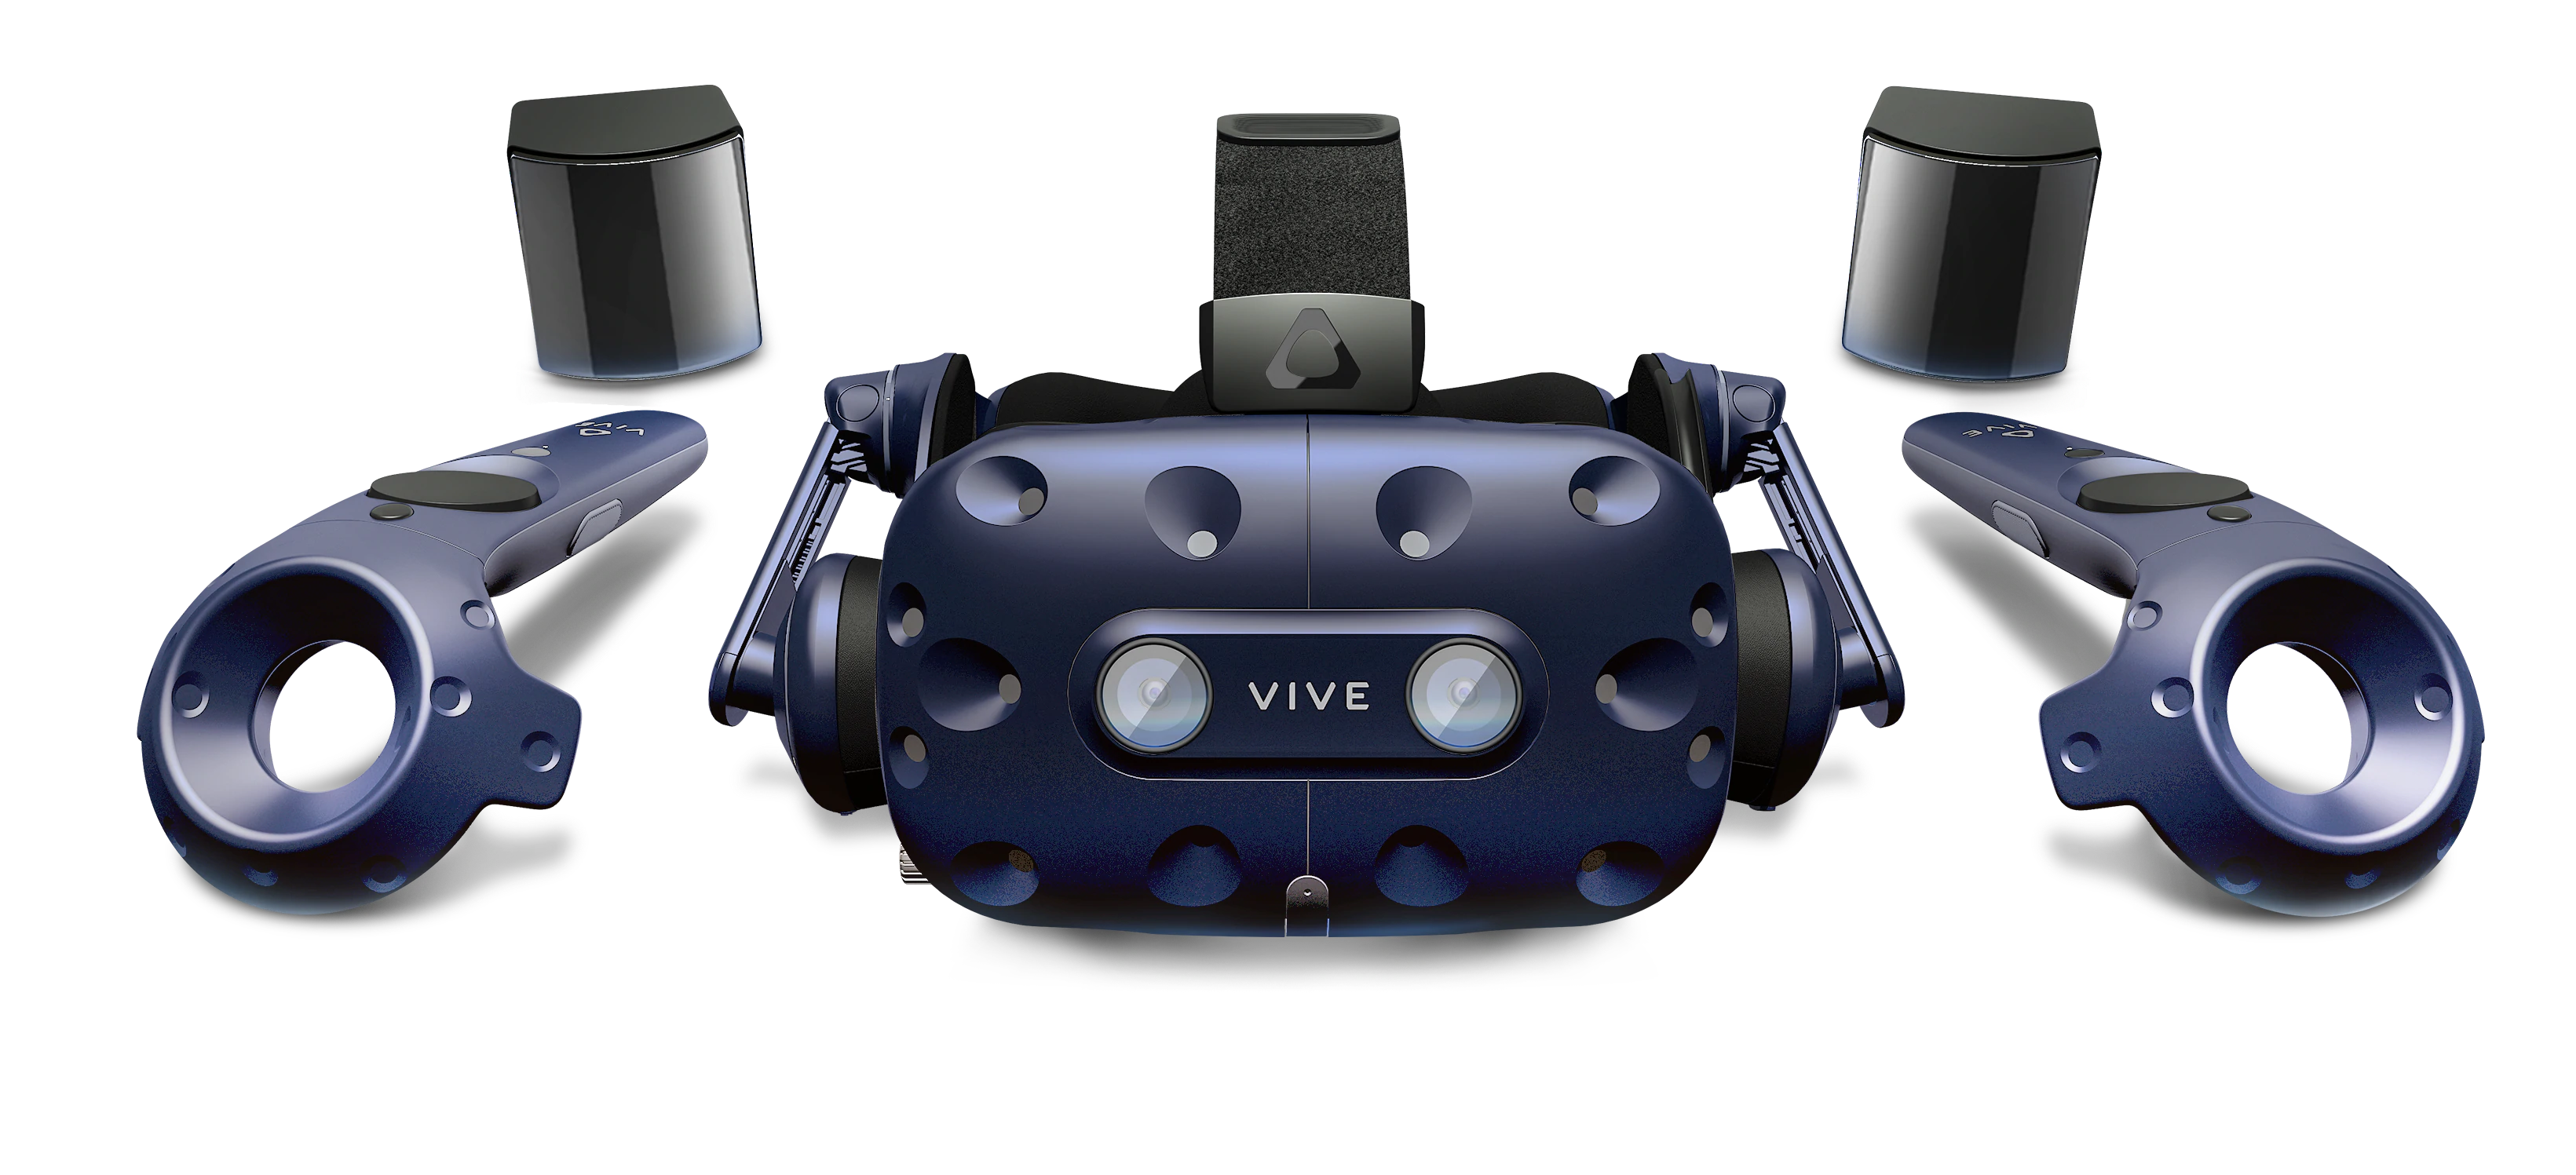
\includegraphics[width=0.7\linewidth]{Bilder/A26_Vivepro}
	\caption{VIVE Pro (mitte), Controller und Basisstationen (außen) [A26]}
	\label{fig:ViveproKit}
\end{figure}
\begin{figure}[h]
	\centering
	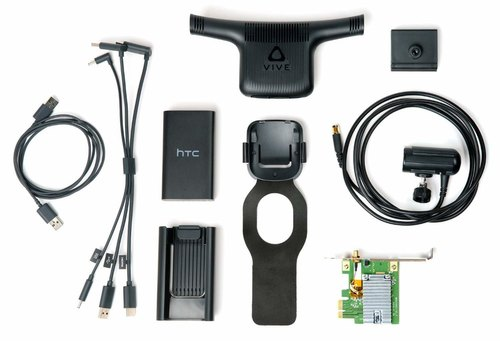
\includegraphics[width=0.5\linewidth]{Bilder/A27_WirelessKit}
	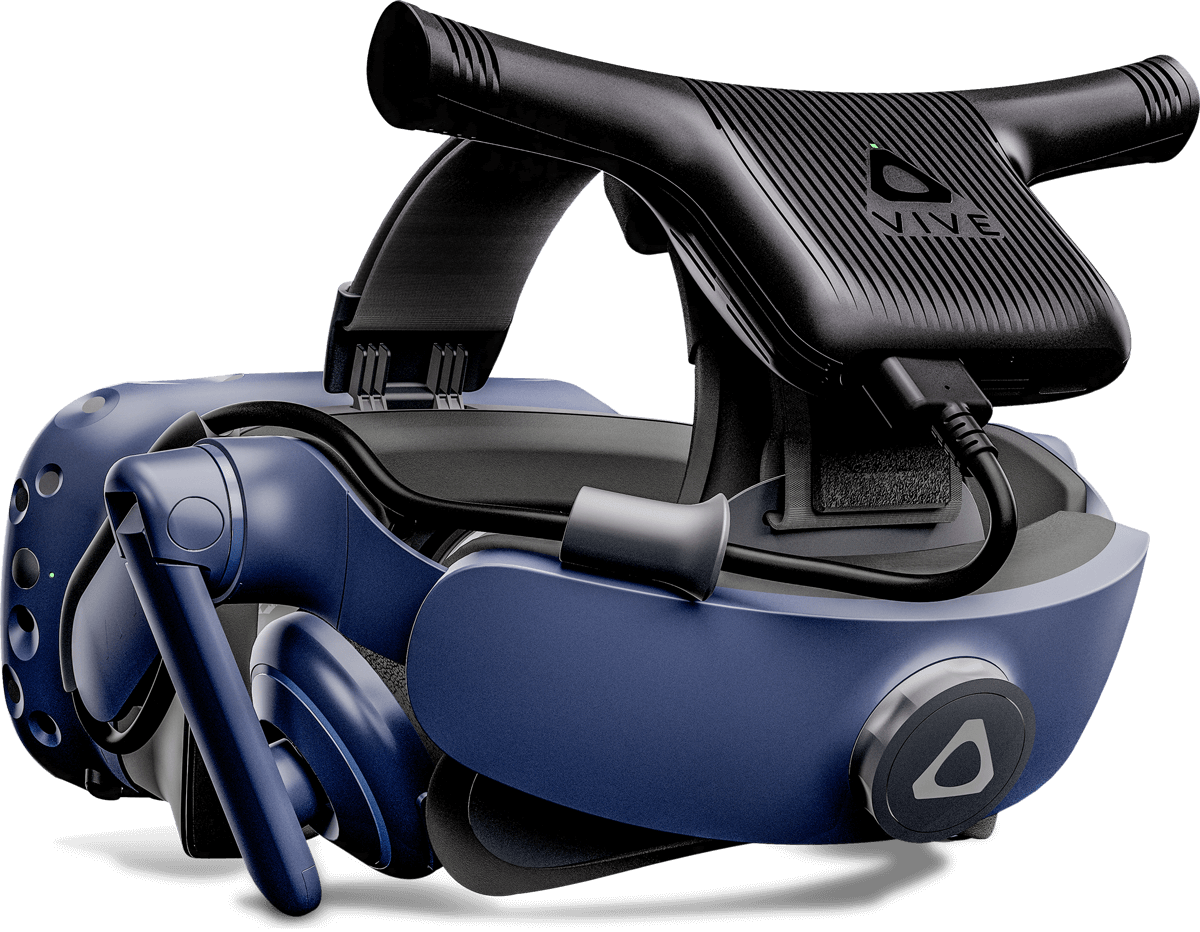
\includegraphics[width=0.4\linewidth]{Bilder/A28_Vive+Wireless}
	\caption{Links: VIVE Wireless Set, inkl. Erweiterungskarte, Sender, Empfänger, Akku, Kabeln und Befestigungen. Rechts: VR Brille mit angeschlossenem Sender. [A27+A28]}
	\label{fig:WirelessKit}
\end{figure}
Neben den außerordentlich guten technischen Spezifikationen der HTC VIVE Pro waren die \textbf{HTC VIVE Tracker} (Vgl. Abbildung \ref{fig:ViveTracker}) ein weiterer Grund warum diese VR Brille zur Umsetzung dieser Arbeit ausgewählt wurde. Die VIVE Tracker werden genauso wie die VR Brille und die dazugehörigen Controller von den Basisstationen im raum geortet und liefern ebenfalls Informationen über ihre Position und Ausrichtung im Raum. Durch den kleinen Formfaktor können die Tracker an beliebigen Objekten befestigt werden um die Bewegung dieser Objekte in der virtuellen Welt abzubilden [30, ViveTracker].
\newline
\begin{figure}[h]
	\centering
	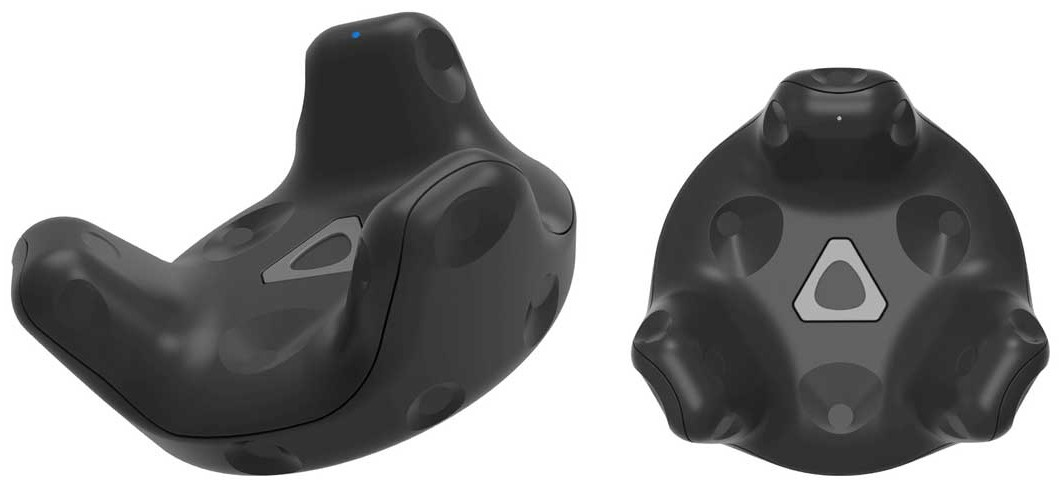
\includegraphics[width=0.5\linewidth]{Bilder/A29_ViveTracker}
	\caption{HTC VIVE Tracker [A29]}
	\label{fig:ViveTracker}
\end{figure}
\newline
Bei dieser Arbeit kamen die Tracker für die Ortung einzelner Körperteile zum Einsatz, da die Hände und der Kopf werden bereits durch die Controller und die VR Brille abgedeckt wurden. Konkret kamen die Tracker für die Ortung der Füße, der Knie, des Beckens und der Ellenbogen zum Einsatz. Durch das Schraubgewinde auf der Unterseite lassen sich die Tracker einfach befestigen. Für die Befestigungen am Becken und an den Füßen wurde auf \textbf{fertige Halterungen} zurückgegriffen (Vgl. Abbildung \ref{fig:Mounts}). Um die Tracker an den Knien und an den Ellenbogen zu befestigen habe ich mir \textbf{eigene Halterungen} gebaut (Vgl. Abbildung \ref{fig:Mounts}). Für diese Halterungen wurden handelsübliche Knie- und Ellenbogenschoner verwendet, durch die ein Loch gebohrt wurde um eine Schraube mit Hilfe einer Mutter zu fixieren. Durch das bereits erwähnte Schraubgewinde auf der Unterseite der Tracker ließen diese sich einfach an diesen Schrauben befestigen.
\begin{figure}[h]
	\centering
	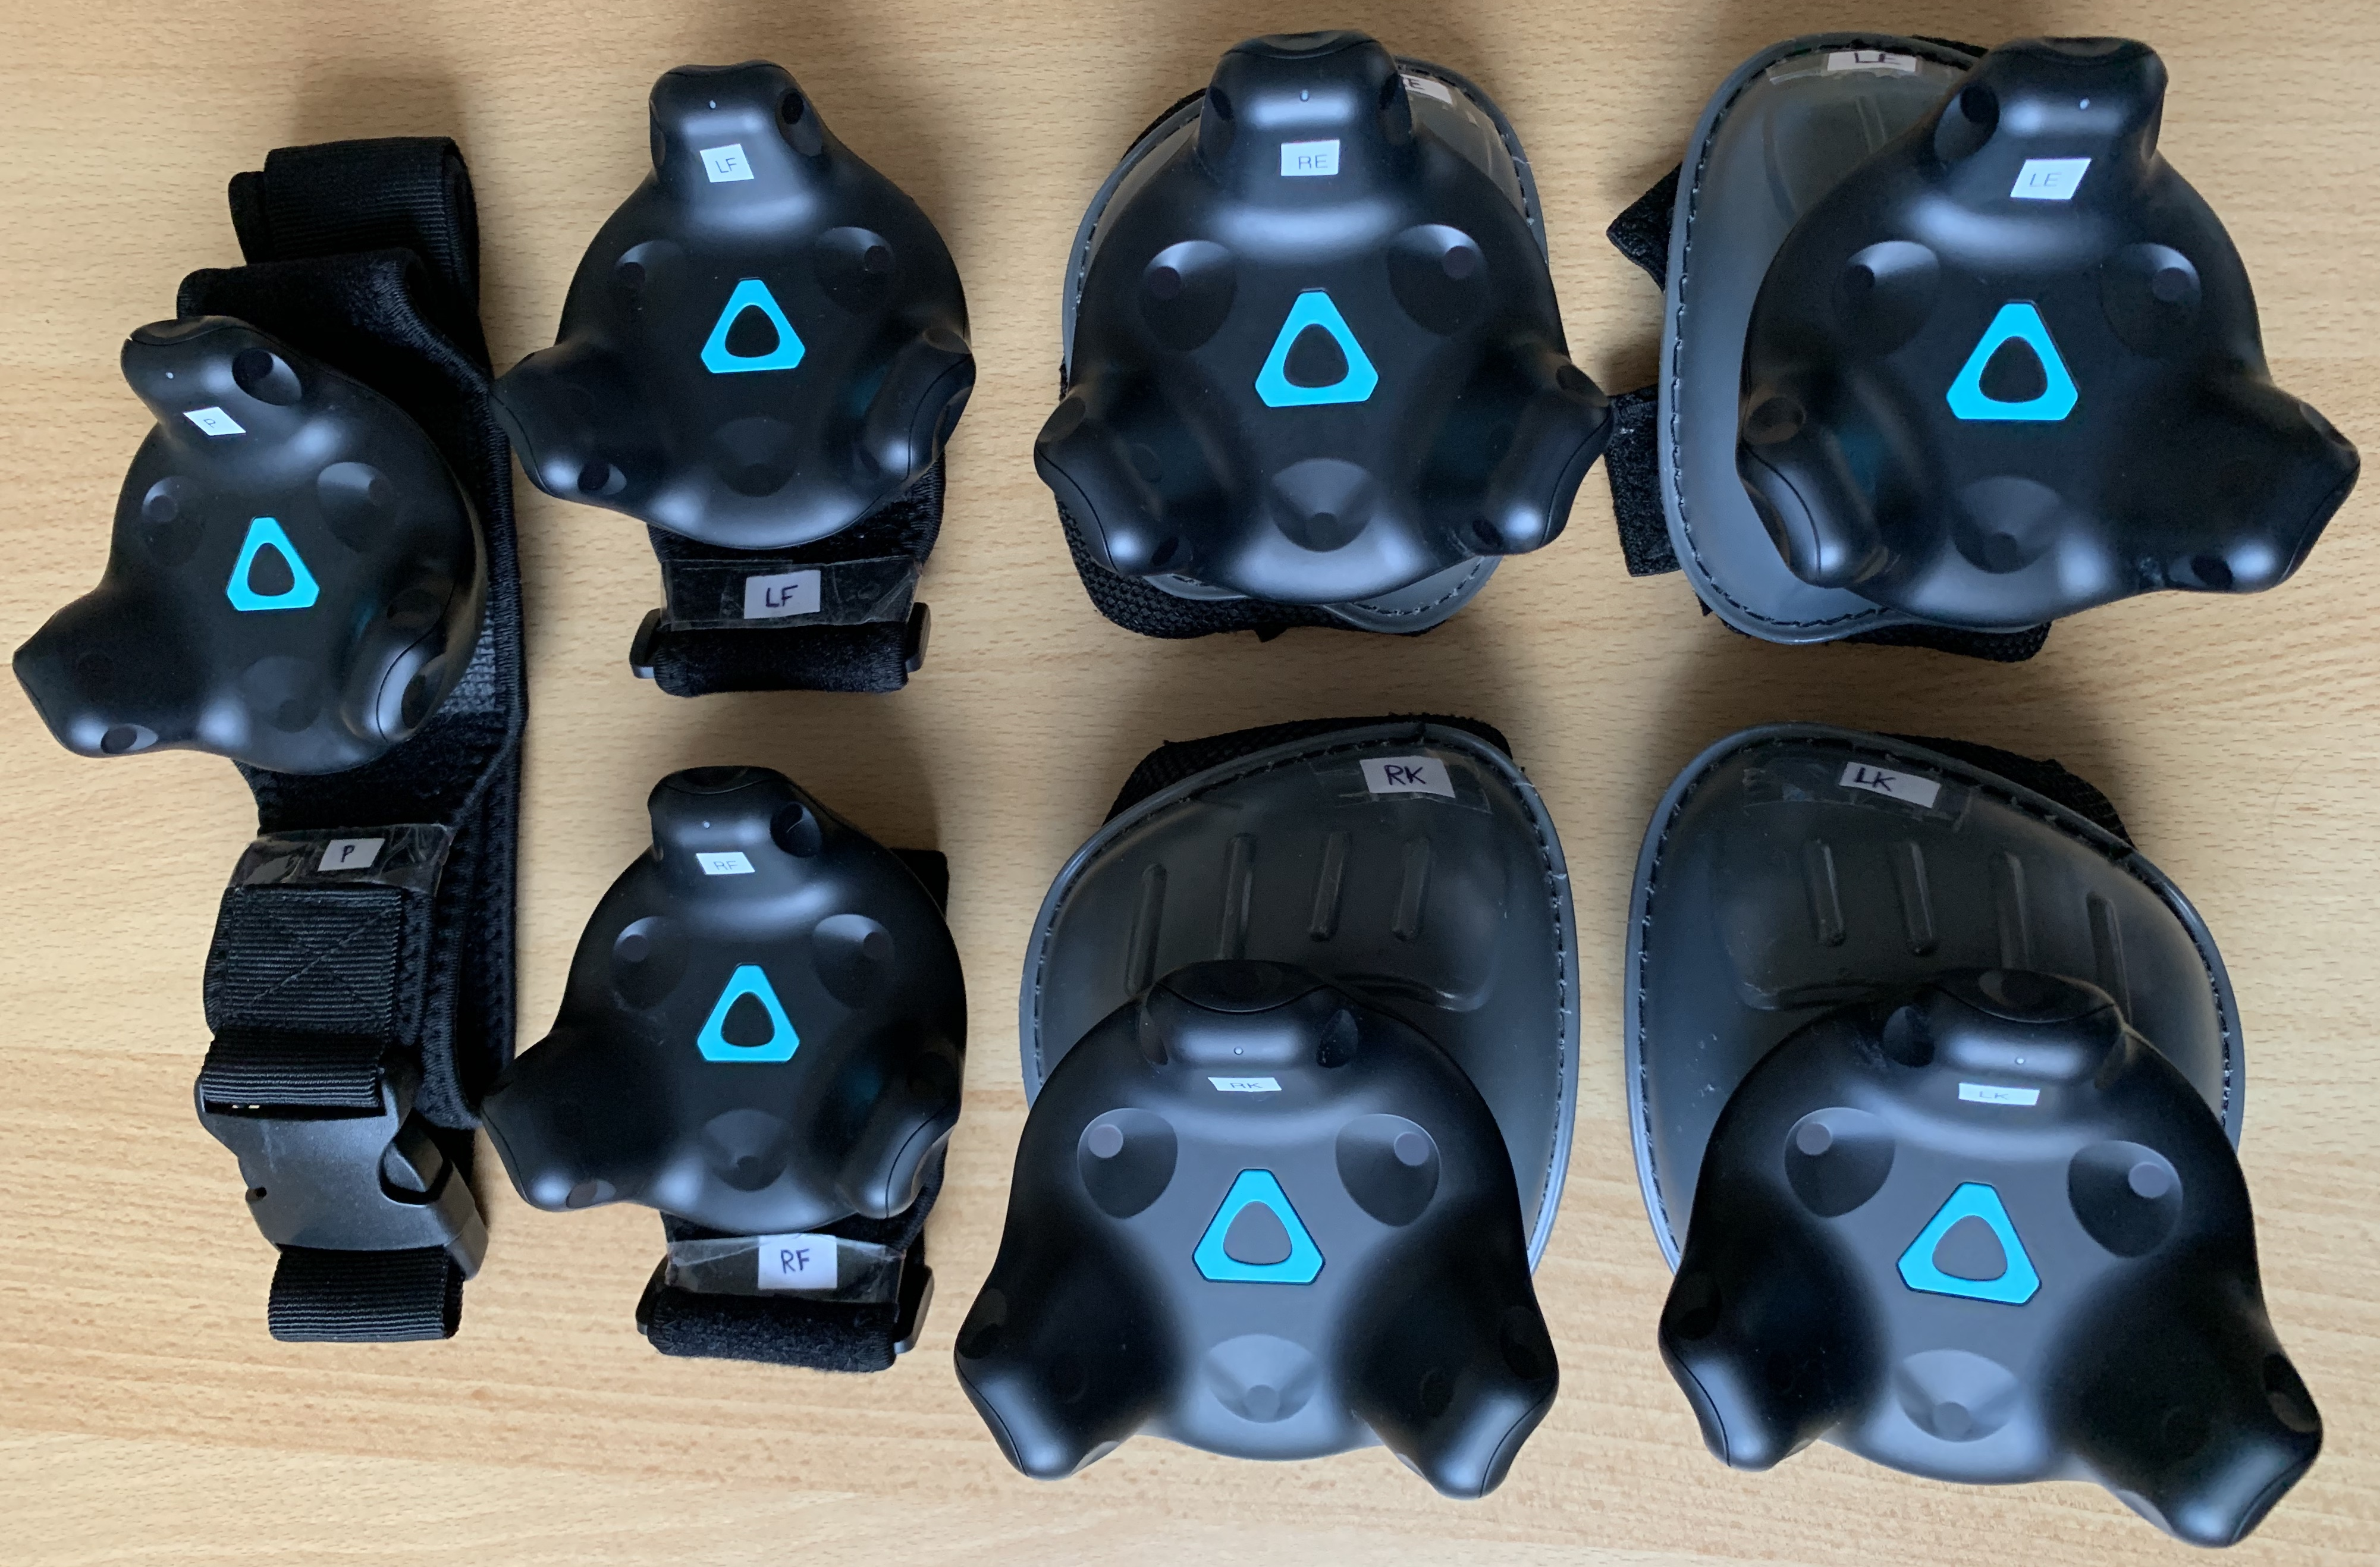
\includegraphics[width=0.7\linewidth]{Bilder/A32_Mounts}
	\caption{Gekaufte (links) und eigene (rechts) Befestigungen für die Tracker, eigene Abbildung}
	\label{fig:Mounts}
\end{figure}

%--------------------------------------------------------------------------------------------------
\section{Eingesetzte Software}\label{sec:Software}
Wie in Abbildung \ref{fig:CodeDarstellung} bereits angedeutet kamen für die Umsetzung dieses Projektes verschiedene Anwendungen und Plugins zum Einsatz. Im Folgenden werden diese genauer erläutert:

\subsection{VIVE Wireless}\label{sec:VIVEWireless}
Die VIVE Wireless Anwendung (Vgl. Abbildung \ref{fig:VIVEWirelessSteamVR}) ist für die direkte Verbindung mit der VR Hardware verantwortlich. Wie bereits in Abbildung \ref{fig:WirelessKit} dargestellt wird dafür im Computer eine Erweiterungskarte installiert, die es einem ermöglicht den entsprechenden Empfänger für die Signale am PC anzuschließen. Der in Abbildung \ref{fig:WirelessKit} dargestellte an der VR Brille montierte Sender bildet das Gegenstück zu diesem Empfänger. Diese Hardware-Erweiterung in Kombination mit der VIVE Wireless Anbindung ermöglicht die kabellose Verwendung der VR Brille.

\subsection{SteamVR}\label{sec:SteamVR}
SteamVR (Vgl. Abbildung \ref{fig:VIVEWirelessSteamVR}) stellt eine weitere wichtige Anwendung im Kontext dieser Arbeit dar. Die meisten Anwendungen für VR Brillen von unterschiedlichen Herstellern sind auf die Schnittstelle der SteamVR Software ausgelegt. Das Gegenstück zu dieser Schnittstelle bildet das SteamVR Plugin, welches im weiteren Verlauf dieses Kapitels vorgestellt wird. Falls die VR Brille ohne das VIVE Wireless Set verwendet wird, wird diese über ein Kabel direkt mit dem PC und somit direkt mit der SteamVR Anwendung verbunden. Da für diese Arbeit das VIVE Wireless Set eingesetzt wurde, wird die VR Brille indirekt über die VIVE Wireless Anwendung mit der SteamVR Anwendung verbunden. Des Weiteren bringt die SteamVR Anwendung eine große Menge an Funktionalitäten mit sich. Dazu gehören Beispielsweise die Möglichkeit den Spielraum zu vermessen oder die Tastenbelegungen der Controller zu verändern. Zusätzlich bietet SteamVR eine Art Hauptmenü an, welches über die in Kapitel \ref{sec:Hardware} angesprochene Taste aufgerufen werden kann.
\newline
Zusammenfassend lässt sich sagen, dass SteamVR eine zentrale Schnittstelle bietet mit der sich die VR Brille, die Controller, die Basisstationen und die Tracker verwalten lassen.
\begin{figure}[h]
	\centering
	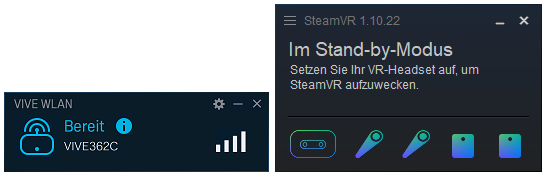
\includegraphics[width=0.8\linewidth]{Bilder/A33_VIVESteam}
	\caption{Links: VIVE Wireless, Rechts: SteamVR, eigene Abbildung}
	\label{fig:VIVEWirelessSteamVR}
\end{figure}

\subsection{Unity Engine}\label{sec:UnitEngine}
Die Unity Engine ist eine 3D-Entwicklungsumgebung und wurde für die Umsetzung dieser Arbeit verwendet. Als Programmiersprache für diese Entwicklungsumgebung kommt die Sprache C\# zum Einsatz.
\newline
Unity bietet den Vorteil in einem Projekt mehrere Szenen (Umgebungen) aufzusetzen und schnell zwischen diesen wechseln zu können. Des Weiteren können die Szenen direkt in der Anwendung bearbeitet werden wenn z.B. 3D-Modelle bearbeitet, hinzugefügt oder entfernt werden sollen. Des Weiteren bringt die Unity Engine eine Vielzahl von bereits eingebauten Funktionalitäten mit sich, die Entwicklern einiges an Arbeit ersparen können. So gibt es Beispielweise vorgefertigte Elemente für grafische Benutzeroberflächen oder sogar ein eingebautes Physiksystem mit dem sich z.B. Kollisionen von Objekten leicht abfragen können. Dank des eingebauten Asset Stores („Marktplatz“) lassen sich in einem internen Marktplatz dank der großen Entwickler-Community aus einer großen Auswahl an Erweiterungen, Texturen, Modelle, etc. beliebig viele Komponenten herunterladen und im eigenen Projekt einfügen. Aufgrund dessen kann man sagen, dass Unity als Entwicklungsumgebung den Entwicklern ermöglicht Modularität in Ihren Projekten umzusetzen.
\newline
Auch bei dieser Arbeit kamen Erweiterungen aus dem Asset Store zum Einsatz. Neben vereinzelten Texturen aus dem Asset Store sind die wichtigsten Erweiterungen das SteamVR und das Final IK Plugin, welche im Folgenden genauer erläutert werden.

\subsubsection{SteamVR Plugin für die Unity Engine}\label{sec:SteamVRPlugin}
Das SteamVR Plugin bildet wie bereits erwähnt und in Abbildung XX illustriert das Gegenstück zur SteamVR Anwendung und vollendet die Schnittstelle zwischen Unity und der VR Hardware. Des Weiteren bietet das Plugin eine große Menge an vorgefertigten Funktionalitäten, wie z.B. das in Abbildung \ref{fig:CodeDarstellung} angedeutete SteamVRTrackedObject Skript.

\subsubsection{Final IK Plugin für die Unity Engine}\label{sec:FinalIKPlugin}
Ein weiteres wichtiges Plugin ist das Final IK Plugin von dem Entwickler RootMotion. Das IK im Namen des Plugins steht für Inverse Kinematics (deutsch: Inverse Kinematik), also „aus vorhandenen Koordinaten Gelenkwinkel berechnen“ [31, Ham., S.20]. Im Kontext dieser Arbeit bedeutet dies, dass mit Hilfe der gelieferten Koordinaten der Tracker die entsprechenden Gelenkwinkel für die Körperteile berechnet werden. Neben diesen Berechnungen liefert das Final IK Plugin noch das eigentliche Modell des Menschen und einige weitere Funktionalitäten, wie z.B. die Kalibrierung des Modells.

%--------------------------------------------------------------------------------------------------
\section{Das Menschmodell}\label{sec:DasMenschmodell}
In diesem Abschnitt zunächst wird der Aufbau und der Nutzen des Menschmodells ohne die Interaktionsschnittstelle erläutert, da diese beiden Komponenten aufgrund der Anforderungen an die Modularität unabhängig voneinander implementiert wurden.

\subsection{Der Aufbau des Menschmodells}\label{sec:MMAufbau}
Das entstandene Menschmodell basiert auf dem durch das Final IK Plugin gelieferten Modells. Im Folgenden werden die einzelnen Komponenten erläutert. Zu den Komponenten gehören das eigentliche Modell, die Skripte und die ergänzenden Komponenten die durch dieser Arbeit dazugekommen sind.

\subsubsection{Das eigentliche Modell}\label{sec:MMModell}
Das Final IK Plugin liefert mehrere Modelle. Für diese Arbeit wurde das Modell mit dem Namen Dummy ausgewählt, welches wie der Name bereits vermuten lässt wie ein Crashtest-Dummy aussieht (Vgl. Abbildung \ref{fig:Dummy}).
\newline\newline
Das Modell in der Szene trägt den Namen \textbf{Dummy} und enthält das sogenannte \textbf{VR IK Skript} des Final IK Plugins. Dieses Skript kümmert sich um die Animation des Modells, daher sind Referenzen zu allen Körperteilen gesetzt. Zu den Körperteilen Kopf, Hände und Füße gibt es zusätzliche Einstellungsmöglichkeiten. Um den Dummy zu verwenden müssen mindestens der Kopf und die beiden Hände als \textbf{Targets} (Ziele für das Tracking) gesetzt werden. Optional können auch die Füße als Targets gesetzt werden. Falls man die Genauigkeit des Trackings um noch eine Stufe verbessern möchte, kann man sogenannte \textbf{Bend Goals} („Beug-Ziele“) setzen (Vgl. Abbildung \ref{fig:TargetBendGoal}). Es gibt insgesamt fünf solcher Bend Goals. Bei dem Kopf ist das zugehörige Bend Goal der Steißbein-Tracker, bei den Händen die Ellenbogen-Tracker und bei den Füßen die Knie-Tracker. Die Targets und Bend Goals werden von dem Skript TrackerAssignment verwaltet, welches im weiteren Verlauf dieses Kapitels erläutert wird.
\begin{figure}[h]
	\centering
	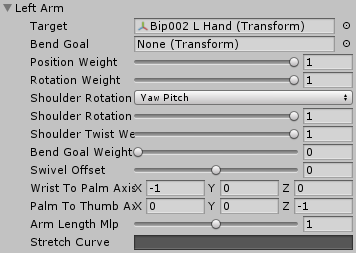
\includegraphics[width=0.4\linewidth]{Bilder/A36_TargetsBendGoals}
	\caption{Targets und Bend Goal am Beispiel des linken Arms, eigene Abbildung}
	\label{fig:TargetBendGoal}
\end{figure}
\newline
Des Weiteren enthält das Objekt Dummy mit dem VR IK Skript zwei weitere Kind-Objekte (Vgl. Abbildung \ref{fig:Dummy}), den \textbf{BipDummy} und den gleichnamigen \textbf{Dummy}. Letzterer ist nur der Skinned-Mesh-Renderer und kümmert sich darum, dass die Texturen der Körperteile gerendert werden. Dies bietet den Vorteil, dass man leicht durch neue Texturen das aussehen des Dummy verändern kann. Das Objekt BipDummy enthält die Transformationen, also Position, Rotation und Skalierung aller Körperteile. Dieser Modulare Aufbau ermöglicht es einem das Menschmodell in Zukunft durch beliebige neue Modelle auszutauschen, solange die Transformationen für die Körperteile Füße, Knie, Steißbein, Hände, Ellenbogen und Kopf vorhanden sind.
\begin{figure}[h]
	\centering
	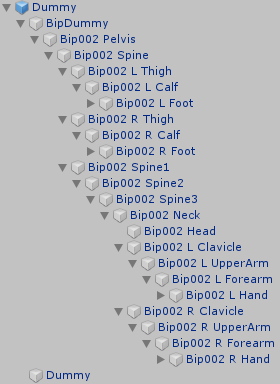
\includegraphics[width=0.4\linewidth]{Bilder/A34_DummyAufbau}
	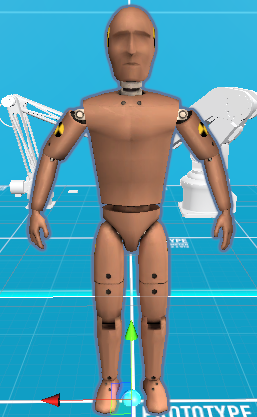
\includegraphics[width=0.338\linewidth]{Bilder/A35_Dummy}
	\caption{Final IK Dummy Modell, eigene Abbildung}
	\label{fig:Dummy}
\end{figure}

\subsubsection{Ergänzende Komponenten}\label{sec:MMKomponenten}
Um das Menschmodell einsatzfähig für die VR Hardware zu machen mussten noch zwei weitere Komponenten zu dem eigentlichen Modell hinzugefügt werden. Diese Komponenten sind das SteamVR CameraRig und die Targets (Ziele) für die optionalen Tracker.
\newline\newline
Das \textbf{SteamVR CameraRig} (Vgl. Abbildung \ref{fig:CameraRig}) ist eine von SteamVR zur Verfügung gestellte Komponente zur Eingrenzung des Spielbereichs und Tracking der Controller (Hier: Hände) und der VR-Brille (Hier: Kopf). Die Komponente besteht aus den drei Kind-Objekten Controller (left), Controler (right) und Camera. Controller (left) und Controller (right) enthalten zusätzlich das 3D-Modell des Controllers als Kind-Objekt, um diesen in der virtuellen Welt anzeigen zu können. 
\newline
Durch diese drei Objekte werden die Bewegungen der beiden Controller und des Kopfes in der virtuellen Welt wiedergespiegelt. Des Weiteren ist es wichtig zu erwähnen, dass das CameraRig für diese Arbeit modifiziert wurde. Den beiden Controllern und der Kamera wurden Kopien der Transformationen der beiden Hände und des Kopfes als Kind-Objekte hinzugefügt. Diese Kopien kamen beim VR IK Skript zum Einsatz um Informationen über die Positionen der Hände und des Kopfes zu erhalten (Vgl. Abbildung \ref{fig:TargetBendGoal}), da diese sich als Kind-Objekte der Controller (Hier: Hände) und der Kamera (Hier: Kopf) entsprechend mitbewegen.
\newline
Abschließend sei noch zu erwähnen, dass die Transformation vom Kopf (Bip002 Head) um ca. -0,113 Einheiten entlang der Y- und Z-Achse gegenüber dem Parent-Objekt Camera verschoben wurde, damit die Kamera sich nicht innerhalb des Kopfes des Modells befindet. Die Transformationen von der linken (Bip002 L Hand) und der rechten (Bip002 R Hand) Hand wurden nicht verschoben.
\begin{figure}[h]
	\centering
	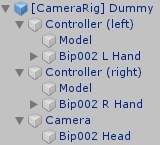
\includegraphics[width=0.25\linewidth]{Bilder/A37_CameraRig}
	\caption{Modifiziertes CameraRig, eigene Abbildung}
	\label{fig:CameraRig}
\end{figure}
\newline
Die zweite wichtige ergänzte Komponente sind die sogenannten \textbf{Targets} (Ziele) (Vgl. Abbildung \ref{fig:Targets}). Da nur sichergestellt ist, dass der Kopf und die Hände durch die VR-Brille und die Controller mit Hilfe des SteamVR CameraRigs verfolgt werden bedarf es zusätzliche Verfolgungsziele für die optionalen Tracker an den Füßen, Knien, Ellenbogen und dem Steißbein.
\newline
Die Targets enthalten momentan noch jeweils ein Kind-Objekt (Vgl. Abbildung \ref{fig:Targets}). Diese Objekte sind lediglich für den Entwicklungsprozess gedacht und können auf Wunsch einfach gelöscht werden, da es sich nur um einfache gefärbte Kugeln handelt, die dem Entwickler anzeigen wo die Tracker sich momentan im Raum befinden. 
\newline
Des Weiteren kommen die Targets genauso wie die Transformationen der Hände und des Kopfes im CameraRig beim VR IK Skript zum Einsatz, um dem Skript Informationen über die Positionen der entsprechenden Körperteile zu liefern. Dabei ist anzumerken, dass die Füße und das Steißbein als eigentliche Targets (Ziele) zum Einsatz kommen, während die Knie und die Ellenbogen als Bend Goals („Beug-Ziele“) verwendet werden (Vgl. Abbildung \ref{fig:TargetBendGoal}).
\begin{figure}[h]
	\centering
	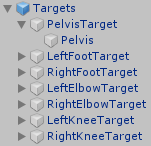
\includegraphics[width=0.25\linewidth]{Bilder/A38_Targets}
	\caption{Targets, eigene Abbildung}
	\label{fig:Targets}
\end{figure}
\newline
Jedes dieser Targets enthält wie bereits in Abbildung \ref{fig:CodeDarstellung} illustriert das Skript \textbf{SteamVR Tracked Object} (Vgl. Abbildung \ref{fig:TrackedObject}). Durch das bereits erwähnte Skript TrackerAssignment wird jedem der Targets der Index des zugehörigen Trackers zugewiesen. Die Standardeinstellung ist „none“, da das Menschmodell auch ohne jegliche dieser optionalen Tracker und sogar nur mit einer beliebigen Teilmenge von ihnen funktioniert.
\begin{figure}[h]
	\centering
	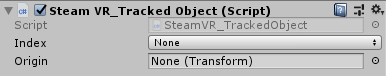
\includegraphics[width=0.45\linewidth]{Bilder/A39_SteamVRTrackedObject}
	\caption{SteamVR Tracked Object Komponente, eigene Abbildung}
	\label{fig:TrackedObject}
\end{figure}

\subsubsection{Ergänzender Code}\label{sec:MMCode}
Für das eigentliche Menschmodell ohne die Interaktionsschnittstelle kommen wie bereits in Abbildung XX dargestellt zwei weitere Klassen zum Einsatz. Diese beiden Klassen tragen die Namen Calibration Controller und TrackerAssignment.
\newline\newline
Die Klasse \textbf{TrackerAssignment} kümmert sich wie bereits erwähnt um die Zuweisung der Tracker zu den entsprechenden Körperteilen. Aufgrund dessen enthält diese Klasse in öffentlichen Variablen Verweise auf alle SteamVR Tracked Object Skripte der optionalen Tracker sowie die Transformationen der zugehörigen Körperteile. Des Weiteren enthält diese Klasse in öffentlichen Variablen Verweise auf den Calibration Controller und das VR IK Skript vom Dummy. Außerdem enthält diese Klasse noch einige private Variablen, insbesondere die bereits in Kapitel XX erwähnten IDs der verschiedenen Tracker.
\newline
Insgesamt enthält diese Klasse zwei Methoden. Die erste Methode trägt den Namen Start und wird wie der Name bereits vermuten lässt einmal bei der Initialisierung ausgeführt und danach nie wieder. In dieser Methode werden lediglich ein paar Variablen die im späteren Verlauf verwendet werden deklariert. Die zweite Methode trägt den Namen AssignTrackers und beinhaltet die gesamte Funktionalität dieser Klasse.
\newline
Zunächst werden mittels einer Schleife alle angeschlossenen Geräte durchlaufen und mit den hinterlegten IDs der Tracker verglichen. Sobald die ID von einem der angeschlossenen Geräte mit einer der hinterlegten IDs übereinstimmt, wird dem SteamVR Tracked Object Skripts des Targets des entsprechenden Körperteils der Index dieses Trackers zugewiesen (Vgl. Abbildung XX).
\newline
Daraufhin werden dem Calibration Controller die Referenzen zu den Transformationen der Füße und des Steißbeins übergeben (Vgl. Abbildung XX), falls diese Tracker aktiv sind. Es ist anzumerken, dass jede beliebige Teilmenge dieser drei Tracker aktiv sein kann, ohne das Ergebnis der Kalibrierung zu verschlechtern.
\newline
Anschließend werden durch den Verweis auf das VR IK Skript die Bend Goals zugewiesen, falls die Tracker für die Knie und Ellenbogen angeschlossen sind. Dafür muss zusätzlich das Bend Goal Weight (die Gewichtung des Bend Goals) auf den Wert 1 gesetzt werden (Vgl. Abbildung XX). Hier ist ebenfalls anzumerken, dass jede beliebige Teilmenge der Tracker aktiv sein kann, ohne das Ergebnis der Darstellung des Menschmodells zu verschlechtern. Falls Beispielsweise der Tracker am linken Ellenbogen aktiv ist aber der Tracker am rechten Ellenbogen nicht, wird die Position des rechten Ellenbogens einfach durch das VR IK Skript anhand der Ausrichtung der Hand und des gesamten Körpers automatisch approximiert.
\newline\newline
Die Klasse \textbf{Calibration Controller} basiert auf dem bereits vorhandenen VR IK Calibrator des Final IK Plugins. Aufgrund dessen enthält die Klasse in öffentlichen Variablen die Verweise auf das VR IK Skript vom Dummy, auf die Transformationen vom Kopf und den beiden Händen und auf die Klasse TrackerAssignment. Des Weiteren enthält die Klasse die öffentlichen Variablen Settings (Einstellungen) und Data (Daten der Kalibrierung). Schließlich enthält die Klasse noch öffentliche aber noch nicht initialisierte Variablen für die Verweise auf die Transformationen des Steißbeins und der beiden Füße.
\newline
Insgesamt enthält die Klasse drei Methoden, wobei die letzte den Namen LateUpdate trägt und in der Regel nicht verwendet wird. Diese Klasse ist nur für Entwicklungszwecke da und war in einer Demo-Klasse des Final IK Plugins vorhanden. Sie ermöglicht es einem die Kalibrierung des Dummys durch das drücken einer bestimmten Taste auf der Tastatur zu starten. Die erste Methode dieser Klasse trägt den Namen Update und wird einmal pro Frame ausgeführt. Aufgabe dieser Methode ist es, sobald vom Bediener die entsprechende Taste am linken Controller gedrückt wird den Kalibrierungsprozess durch die zweite Methode der Klasse mit dem Namen Calibrate zu starten. Es ist anzumerken, dass der Kalibrierungsprozess beliebig oft ausgeführt und somit nach Bedarf erneuert werden kann.
\newline
In der Methode Calibrate wird zunächst durch den Verweis auf die Klasse TrackerAssignment die Zuweisung der einzelnen Tracker gestartet. Hierbei ist anzumerken, dass wie bereits vorher erwähnt und in Abbildung XX dargestellt die noch nicht initialisierten Variablen für die Verweise auf die Transformationen des Steißbeins und der beiden Füße initialisiert werden, falls die entsprechenden Tracker angeschlossen sind. Ansonsten werden für die Kalibrierung lediglich die Positionen der Hände und des Kopfes berücksichtigt. In jedem Fall werden für die Kalibrierung die Positionen der Knie und der Ellenbogen nicht berücksichtigt.
\newline
Schließlich wird der eigentliche Kalibrierungsprozess durch die gleichnamige Methode Calibrate der Klasse VR IK Calibrator gestartet, indem die entsprechenden Variablen an diese Methode übergeben werden. Die vorher angesprochenen Variablen Settings und Data sind dafür da, falls man der Methode mit Hilfe der Klasse VR IK Calibrator und deren Methoden Kalibrierungen abspeichern und wieder laden möchte. Diese Funktionalität wurde für diese Arbeit nicht berücksichtigt.




\subsection{Funktionalitäten des Menschmodells}\label{sec:MMFunktionen}
%--------------------------------------------------------------------------------------------------
\section{Die Interaktion}\label{sec:DieInteraktion}



